%%%%%%%%%%%%%%%%%%%%%%%%%%%%%%%%%%%%%%%%%%%%%%%%%%%%%%%%%%%%%%%%%%%%%%%%%%%%%%%%
% Soutenance de projet - Fichier modèle pour présentations Beamer
%%%%%%%%%%%%%%%%%%%%%%%%%%%%%%%%%%%%%%%%%%%%%%%%%%%%%%%%%%%%%%%%%%%%%%%%%%%%%%%%
\documentclass{beamer}
\usepackage[utf8]{inputenc}
\usepackage[francais]{babel}
\usepackage[T1]{fontenc}
\usepackage{textcomp}
\usepackage{relsize}
\usepackage{amssymb}
\usepackage{framed}
% \usepackage{makeidx}


%%% THÈME TORINO AVEC MINIFRAMES MODIFIÉES - NÉCESSITE FICHIERS SPÉCIAUX
\usetheme[pageofpages=sur,% String used between the current page and the
                         % total page count.
          alternativetitlepage=true,% Use the fancy title page.
          titlepagelogo=logo,% Logo for the first page.
          titleline=true,
          watermark=watermark,% Watermark used in every page.
          watermarkheight=100px,% Height of the watermark.
          watermarkheightmult=4,% The watermark image is 4 times bigger
                                % than watermarkheight.
          ]{Torino}
\useoutertheme[subsection=true]{miniframes2}
\usecolortheme{freewilly}
%%% FIN DU SECOND THÈME

% Add images path to graphics default include path
\graphicspath{{images/}}

% nouvelle commande pour un joli nom
\newcommand{\nom}[1]{\textsc{#1}}

% commande pour une zolie ligne
\newcommand{\ligne}[1][1pt]{
  \par\noindent
  \rule[.5ex]{\linewidth}{#1}\par}

% \0
\newcommand{\slz}{$\backslash0$}

\newcommand{\executeiffilenewer}[3]{%
 \ifnum\pdfstrcmp{\pdffilemoddate{#1}}%
 {\pdffilemoddate{#2}}>0%
 {\immediate\write18{#3}}\fi%
}

\newcommand{\includesvg}[2]{%
 \executeiffilenewer{#1.svg}{#1.pdf}%
 {inkscape -z -D --file=#1.svg --export-pdf=#1.pdf --export-width=1000}%
% \input{#1.eps_tex}%
 \includegraphics[scale=#2]{#1.pdf}
}

\newcommand{\includedot}[2]{%
 \executeiffilenewer{#1.dot}{#1.pdf}%
 {dot -T pdf -o #1.pdf #1.dot}%
 %\input{#1.eps_tex}%
 \includegraphics[scale=#2]{#1.pdf}
}

\newcommand{\includepic}[2]{%
 \immediate\write18{pic2plot -Tsvg --bg-color none #1.pic > #1.svg && inkscape -z -D --file=#1.svg --export-pdf=#1.pdf --export-width=1000}%
 \includegraphics[scale=#2]{#1.pdf}
}

%%% TITRE DE PAGE
\title{\huge Intégration de PIGA dans le noyau Linux}
\subtitle{\Large Projet recherche 2011 -- 2012}
\author{\Large Timothée~Ravier}
\institute{ENSI de Bourges}
\date{10 février 2012}

%%% POUR AVOIR UN PLAN QUI S'AFFICHE QUAND ON CHANGE DE SOUS-SECTION
\AtBeginSection[ ]
{
 \begin{frame}<beamer>
   \frametitle{Plan}
   \tableofcontents[currentsection]
  \end{frame}
}
\NoAutoSpaceBeforeFDP

\begin{document}

%%% LA PAGE DE TITRE, ON PEUT Y APPLIQUER DES OPTIONS COMME INSTITUTE CI-DESSOUS
{
	\framenumberoff
	\watermarkoff
	\institute{École Nationale Supérieure d'Ingénieurs de Bourges} % Vire le champ institut sur cette page
	\begin{frame}
	\titlepage
	\end{frame}
}

\section{Architecture}
\begin{frame}{SELinux et PIGA}
	Principe d'une protection système avancée
	\begin{itemize}
		\item Propriétés de sécurité évoluées
		\item Base de signatures
		\item Contrôle de ces activités
	\end{itemize}
	\vspace{-1cm}
	\hspace{1cm}
		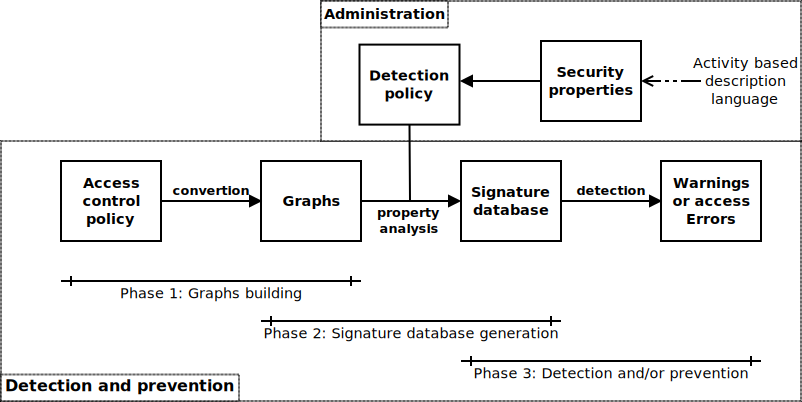
\includegraphics[scale=0.22]{modele_generale_en.pdf}
\end{frame}

\begin{frame}{De PIGA-IDS/IPS à PIGA-Linux}
	\begin{center}
		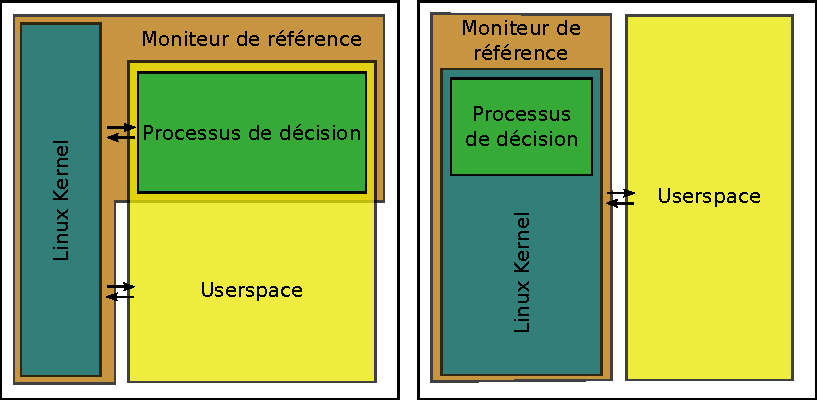
\includegraphics[scale=0.8]{piga_evol.pdf}
	\end{center}
	\vspace{-0.5cm}
	\begin{itemize}
		\item meilleures performances
		\item robustesse (attaques sur le moniteur de référence plus
difficile)
	\end{itemize}
\end{frame}

\section{Intégration dans le noyau}
\begin{frame}{Dissocier le stockage et la progression}
	\begin{itemize}
		\item Architecture générique
		\item Simplification de la communication avec l'espace utilisateur
		\item Possibilité d'implémentations multiples
		\item Travail encore en cours (non fonctionnel)
	\end{itemize}
\end{frame}

\begin{frame}{Implémentation générique}
	Complexité linaire en fonction de la taille des données entrées :
	\begin{itemize}
		\item le tri et l'efficacité reposent sur l'organisation et l'algorithme
de recherche dans le moyen de stockage
	\end{itemize}
\end{frame}

\begin{frame}{Verrous et accès concurrent}
	\begin{itemize}
		\item 
		\item 
	\end{itemize}
\end{frame}

\begin{frame}{Difficultés liées au crochets LSM}
	\begin{itemize}
		\item Définition ponctuelle des crochets LSM
		\item Pas de prise en compte ni la durée ni de la date de fin d'une
intéraction
		\item Ne correspond pas au modèle théorique de PIGA
	\end{itemize}
\end{frame}

% \begin{frame}{}
% 	\begin{itemize}
% 		\item 
% 		\item 
% 		\item 
% 	\end{itemize}
% \end{frame}

\section{Démonstration}
\begin{frame}
	\frametitle{Démonstration}
\end{frame}

\end{document}
